\documentclass{article}
\usepackage{amsmath}
\usepackage{amsfonts}
\usepackage{geometry}
\usepackage{xcolor}
\usepackage{tikz}
\usepackage{pgfplots} % For creating graphs
\pgfplotsset{compat=1.18}
\usetikzlibrary{shapes.geometric, arrows, positioning}
\usepackage{listings} % For code syntax highlighting
\usepackage{xcolor} % Already included but ensure for listings

% Configure TypeScript syntax highlighting
\lstdefinelanguage{TypeScript}{
  keywords={const, let, var, function, return, if, else, for, while, break, continue, true, false, null, undefined, number, string, boolean, any, void, interface, type, class, extends, implements, public, private, protected, static, readonly, abstract, async, await, import, export, from, as, default},
  keywordstyle=\color{blue}\bfseries,
  ndkeywords={console, log},
  ndkeywordstyle=\color{purple}\bfseries,
  identifierstyle=\color{black},
  sensitive=true,
  comment=[l]{//},
  morecomment=[s]{/*}{*/},
  commentstyle=\color{gray}\ttfamily,
  stringstyle=\color{red}\ttfamily,
  morestring=[b]',
  morestring=[b]",
  morestring=[b]`,
}

\lstset{
  language=TypeScript,
  basicstyle=\ttfamily\footnotesize,
  numbers=left,
  numberstyle=\tiny\color{gray},
  stepnumber=1,
  numbersep=5pt,
  backgroundcolor=\color{gray!5},
  showspaces=false,
  showstringspaces=false,
  showtabs=false,
  frame=single,
  rulecolor=\color{black},
  tabsize=2,
  captionpos=b,
  breaklines=true,
  breakatwhitespace=false,
  escapeinside={\%*}{*\%},
  aboveskip=\bigskipamount,
  belowskip=\bigskipamount
}
\geometry{margin=1in}

% Define a command for code variables
\newcommand{\code}[1]{\textcolor{blue}{\texttt{#1}}}

\title{Energy Calculations for PTAC vs PTHP Systems}
\author{EDK Energy Insight Platform}
\date{\today}

\begin{document}

\maketitle

\section{Introduction}

This document outlines the energy calculations for comparing Packaged Terminal Air Conditioner (PTAC) and Packaged Terminal Heat Pump (PTHP) systems, using the standardized variable names from our codebase.

\section{PTAC System Calculations}

\subsection{Per-Unit Constants}

The system uses fundamental constants for PTAC units in original units and their MMBtu equivalents:

\begin{itemize}
    \item \code{annualUnitThermsHeatingPTAC}: 255 therms per year per unit for heating
    \item \code{annualUnitKwhCoolingPTAC}: 16,000 kWh per year per unit for cooling
    \item \code{annualUnitMMBtuHeatingPTAC}: 25.5 MMBtu per year per unit for heating
        \begin{itemize}
            \item Converted from 255 therms × 0.1 MMBtu/therm = 25.5 MMBtu
        \end{itemize}
    \item \code{annualUnitMMBtuCoolingPTAC}: 5.459427 MMBtu per year per unit for cooling
        \begin{itemize}
            \item Converted from 16,000 kWh × 0.003412 MMBtu/kWh = 5.459427 MMBtu
        \end{itemize}
\end{itemize}

\subsection{Building-Level Calculations}

For a building with multiple units, we calculate both MMBtu and original unit values:

\subsubsection{MMBtu Building Totals}
\begin{equation}
\code{annualBuildingMMBtuCoolingPTAC} = N_{ptacUnits} \times \code{annualUnitMMBtuCoolingPTAC}
\end{equation}

\begin{equation}
\code{annualBuildingMMBtuHeatingPTAC} = N_{ptacUnits} \times \code{annualUnitMMBtuHeatingPTAC}
\end{equation}

\begin{equation}
\code{annualBuildingMMBtuTotalPTAC} = \code{annualBuildingMMBtuCoolingPTAC} + \code{annualBuildingMMBtuHeatingPTAC}
\end{equation}


\section{PTHP System Calculations}

\subsection{Heating Energy Conversion with Building-Specific EFLH}

For PTHP systems, the heating energy is calculated using building-specific Equivalent Full Load Hours (EFLH) derived from PLUTO data, combined with PTHP heating capacity and coefficient of performance:

\subsubsection{Step 1: Calculate Annual Building kWh for PTHP Heating}

The annual building heating consumption in kWh is calculated using the detailed equation:

\begin{equation}
\code{annualBuildingkWhHeatingPTHP} = \frac{\code{heatingCapacityPTHP}}{3.412} \times \frac{1}{\code{pthpCOP}} \times \text{EFLH} \times N_{ptacUnits}
\end{equation}

Where:
\begin{itemize}
    \item \code{heatingCapacityPTHP}: 8 KBtu (constant heating capacity per PTHP unit)
    \item 3.412: Conversion factor from KBtu to kW (kW per KBtu)
    \item \code{pthpCOP}: 1.51 (Coefficient of Performance for PTHP)
    \item EFLH: Equivalent Full Load Hours (building-specific, from PLUTO data)
    \item $N_{ptacUnits}$: Number of PTAC units to be replaced
\end{itemize}

\subsubsection{Step 2: EFLH Lookup from PLUTO Data}

The EFLH value is determined by building characteristics from PLUTO data using the following function:

\begin{lstlisting}
export function getEFLHFromPluto(yearBuilt: number | string, floors: number | string): number {
  const [year, numFloors] = [Number(yearBuilt), Number(floors)];
  if (!Number.isFinite(year) || year <= 0 || !Number.isFinite(numFloors) || numFloors <= 0) {
    throw new Error(`Invalid inputs: yearBuilt=${yearBuilt}, floors=${floors}`);
  }

  const buildingType = numFloors <= 6 ? "LOW_RISE" : "HIGH_RISE";
  const constructionEra = year <= 1939 ? "PREWAR" :
                         year <= 1978 ? "PRE79" :
                         year <= 2006 ? "1979_2006" : "2007PRESENT";

  const eflhTable = {
    LOW_RISE: {
      PREWAR: 974,
      PRE79: 738,
      "1979_2006": 705,
      "2007PRESENT": 491
    },
    HIGH_RISE: {
      PREWAR: 987,
      PRE79: 513,
      "1979_2006": 385,
      "2007PRESENT": 214
    }
  };
  
  return eflhTable[buildingType][constructionEra];
}
\end{lstlisting}

The EFLH table categorizes buildings by:
\begin{itemize}
    \item \textbf{Building Type}: Low-rise ($\leq$ 6 floors) vs High-rise (> 6 floors)
    \item \textbf{Construction Era}: Pre-war ($\leq$ 1939), Pre-79 (1940-1978), 1979-2006, 2007-Present
    \item \textbf{EFLH Range}: 214-987 hours depending on building characteristics
\end{itemize}

\subsubsection{Step 3: Convert kWh to MMBtu}

Finally, convert the kWh result to MMBtu for consistency with other calculations:

\begin{equation}
\code{annualBuildingMMBtuHeatingPTHP} = \code{annualBuildingkWhHeatingPTHP} \times 0.003412
\end{equation}

Where 0.003412 is the conversion factor from kWh to MMBtu.

\subsection{Cooling Energy}

The cooling energy for PTHP remains equivalent to PTAC:

\begin{equation}
\code{annualBuildingMMBtuCoolingPTHP} = \code{annualBuildingMMBtuCoolingPTAC}
\end{equation}

\subsection{Total PTHP Energy}

The total annual building energy consumption for PTHP:

\begin{equation}
\code{annualBuildingMMBtuTotalPTHP} = \code{annualBuildingMMBtuCoolingPTHP} + \code{annualBuildingMMBtuHeatingPTHP}
\end{equation}

\subsection{PTHP Building Totals for Cost Calculations}

\begin{equation}
\code{annualBuildingKwhHeatingPTHP} = N_{ptacUnits} \times \code{annualUnitKwhHeatingPTHP}
\end{equation}

\begin{equation}
\code{annualBuildingKwhCoolingPTHP} = N_{ptacUnits} \times \code{annualUnitKwhCoolingPTHP}
\end{equation}

\section{Energy Reduction Analysis}

The energy reduction achieved by switching from PTAC to PTHP is calculated as:

\begin{equation}
\text{Reduction (\%)} = \frac{\code{annualBuildingMMBtuTotalPTAC} - \code{annualBuildingMMBtuTotalPTHP}}{\code{annualBuildingMMBtuTotalPTAC}} \times 100\%
\end{equation}

\section{Total Retrofit Cost Calculation}

The total cost for retrofitting from PTAC to PTHP systems includes unit costs, installation costs, and contingency:

\begin{equation}
\code{totalRetrofitCost} = (\code{pthpUnitCost} + \code{pthpInstallationCost}) \times \text{Total PTHP Units} \times (1 + \code{pthpContingency})
\end{equation}

Example calculation:
\begin{equation}
\code{totalRetrofitCost} = (\$1,100 + \$450) \times N_{ptacUnits} \times 1.10 = \$1,705 \times N_{ptacUnits}
\end{equation}

Where:
\begin{itemize}
    \item \code{pthpUnitCost}: \$1,100 per PTHP unit
    \item \code{pthpInstallationCost}: \$450 per unit
    \item \code{pthpContingency}: 10\% (1.10 multiplier)
    \item $N_{ptacUnits}$: Total number of PTHP units to be installed
\end{itemize}

\section{Energy Cost Savings Calculation}

The building energy totals for PTAC need to be expressed in kWh and therms so we can calculate price:

\begin{equation}
\code{annualBuildingThermsHeatingPTAC} = N_{ptacUnits} \times \code{annualUnitThermsHeatingPTAC}
\end{equation}

\begin{equation}
\code{annualBuildingKwhCoolingPTAC} = N_{ptacUnits} \times \code{annualUnitKwhCoolingPTAC}
\end{equation}

The annual energy cost savings from switching to PTHP systems is calculated as:

\begin{align}
\code{annualBuildingCostPTAC} &= \code{annualBuildingKwhCoolingPTAC} \times \code{priceKwhHour} \nonumber \\
&\quad + \code{annualBuildingThermsHeatingPTAC} \times \code{priceThermHour}
\end{align}

\begin{align}
\code{annualBuildingCostPTHP} &= \code{annualBuildingKwhHeatingPTHP} \times \code{priceKwhHour} \nonumber \\
&\quad + \code{annualBuildingKwhCoolingPTHP} \times \code{priceKwhHour}
\end{align}

\begin{align}
\code{annualSavingsEnergy} &= \code{annualBuildingCostPTAC} - \code{annualBuildingCostPTHP}
\end{align}

Where:
\begin{itemize}
    \item \code{priceKwhHour}: \$0.24 per kilowatt-hour for electricity (NYC average)
    \item \code{priceThermHour}: \$1.45 per therm for natural gas (NYC average)\footnote{Heating oil is priced at \$2.60-\$2.77 per therm, but most buildings use natural gas.}
\end{itemize}

\section{LL97 Emissions Savings and BE Credit}

\subsection{Current Building Emissions and Budget}

The building's current emissions are obtained from LL84 reporting:

\begin{align}
\code{totalBuildingEmissionsLL84} &= \text{Current building emissions (metric tons CO2e)}
\end{align}

The emissions budget for the building is calculated as the sum of type-specific emissions limits applied to corresponding square footage\footnote{Key LL97 property type limits (tCO2e/sf): Office (2024-29: 0.00846, 2030-34: 0.00453), Retail Store (2024-29: 0.01582, 2030-34: 0.00775), Multifamily Housing (2024-29: 0.00892, 2030-34: 0.00453), Hotel (2024-29: 0.01344, 2030-34: 0.00775), Hospital (2024-29: 0.02551, 2030-34: 0.01542), K-12 School (2024-29: 0.00846, 2030-34: 0.00453), Warehouse (2024-29: 0.00404, 2030-34: 0.00297). Complete mapping available in codebase at src/ll97/ll97\_espm\_to\_bc\_caps.json.}:

\begin{align}
\code{emissionsBudget} &= \sum_{i} \code{squareFootageByType}_i \times \code{emissionsLimit}_i
\end{align}

\subsection{Current Fee Calculation}

LL97 has two compliance periods with different emissions budgets. The annual fee for exceeding the emissions budget is calculated separately for each period:

\subsubsection{2024-2029 Compliance Period}
\begin{align}
\code{emissionsBudget2024to2029} &= \sum_{i} \code{squareFootageByType}_i \times \code{emissionsLimit2024to2029}_i
\end{align}

\begin{align}
\code{annualFeeExceedingBudget2024to2029} &= (\code{totalBuildingEmissionsLL84} \nonumber\\
&\quad - \code{emissionsBudget2024to2029}) \times \code{feePerTonCO2e}
\end{align}

\subsubsection{2030-2034 Compliance Period}
\begin{align}
\code{emissionsBudget2030to2034} &= \sum_{i} \code{squareFootageByType}_i \times \code{emissionsLimit2030to2034}_i
\end{align}

\begin{align}
\code{annualFeeExceedingBudget2030to2034} &= (\code{totalBuildingEmissionsLL84} \nonumber\\
&\quad - \code{emissionsBudget2030to2034}) \times \code{feePerTonCO2e}
\end{align}

Where \code{feePerTonCO2e} = \$268 per tCO2e over budget, and the 2030-2034 period has more stringent (lower) emissions limits than the 2024-2029 period.

\subsection{BE Credit Section (Beneficial Electrification)}

\subsubsection{BE Credit Calculation}

The BE credit is calculated based on heating electrification only, using annual heating kWh and time-dependent coefficients:

\begin{align}
\code{beCreditBefore2027} &= \code{annualBuildingkWhHeatingPTHP} \times 0.0013
\end{align}

\begin{align}
\code{beCredit2027to2029} &= \code{annualBuildingkWhHeatingPTHP} \times 0.00065
\end{align}

Where:
\begin{itemize}
    \item Before January 1, 2027: Coefficient = 0.0013 tCO₂e/kWh
    \item 2027-2029: Coefficient = 0.00065 tCO₂e/kWh
\end{itemize}

\subsubsection{Adjusted Building Emissions Calculation}

To accurately assess the LL97 fee impact of the PTAC→PTHP retrofit, we must calculate the building's adjusted emissions that reflect the actual post-retrofit energy consumption and emissions profile, rather than using the baseline LL84 emissions\footnote{Using raw LL84 emissions would not account for the actual emissions reduction from switching from gas heating to electric heat pumps, which varies by time period due to changing grid electricity emissions factors.}.

The adjusted building emissions are calculated as:

\begin{align}
\code{adjustedTotalBuildingEmissions} &= \code{totalBuildingEmissionsLL84} \nonumber \\
&\quad - (\code{annualBuildingMMBtuHeatingPTAC} \times \code{efGas}) \nonumber \\
&\quad + (\code{annualBuildingKwhHeatingPTHP} \times \code{efGrid\_kWh(year)})
\end{align}

Where the emissions factors are:
\begin{itemize}
    \item \code{efGas}: 0.05311 tCO₂e/MMBtu (natural gas factor, constant 2024-2034)
    \item \code{efGrid\_kWh(year)}: Grid electricity factor (tCO₂e/kWh) varying by compliance period:
    \begin{itemize}
        \item \code{efGrid2024to2029}: 0.000288962 tCO₂e/kWh
        \item \code{efGrid2030to2034}: 0.000145 tCO₂e/kWh
    \end{itemize}
\end{itemize}

This gives us period-specific adjusted emissions:

\begin{align}
\code{adjustedTotalBuildingEmissions2024to2029} &= \code{totalBuildingEmissionsLL84} \nonumber \\
&\quad - (\code{annualBuildingMMBtuHeatingPTAC} \times 0.05311) \nonumber \\
&\quad + (\code{annualBuildingKwhHeatingPTHP} \times 0.000288962)
\end{align}

\begin{align}
\code{adjustedTotalBuildingEmissions2030to2034} &= \code{totalBuildingEmissionsLL84} \nonumber \\
&\quad - (\code{annualBuildingMMBtuHeatingPTAC} \times 0.05311) \nonumber \\
&\quad + (\code{annualBuildingKwhHeatingPTHP} \times 0.000145)
\end{align}

\subsubsection{Annual Fee with BE Credit (Before 2027)}

For buildings upgrading before January 1, 2027:

\begin{align}
\code{newEmissionsBefore2027} &= \code{adjustedTotalBuildingEmissions2024to2029} - \code{beCreditBefore2027}
\end{align}

\begin{align}
\code{adjustedAnnualFeeBefore2027} &= (\code{newEmissionsBefore2027} \nonumber\\
&\quad - \code{emissionsBudget2024to2029}) \times \code{feePerTonCO2e}
\end{align}

\subsubsection{Annual Fee with BE Credit (2027-2029)}

For buildings upgrading between 2027-2029:

\begin{align}
\code{newEmissions2027to2029} &= \code{adjustedTotalBuildingEmissions2024to2029} - \code{beCredit2027to2029}
\end{align}

\begin{align}
\code{adjustedAnnualFee2027to2029} &= (\code{newEmissions2027to2029} \nonumber\\
&\quad - \code{emissionsBudget2024to2029}) \times \code{feePerTonCO2e}
\end{align}

\subsubsection{Annual Fee for 2030-2034}

For the 2030-2034 period, there is no BE credit available, so the fee is calculated using the adjusted emissions for this period:

\begin{align}
\code{adjustedAnnualFee2030to2034} &= (\code{adjustedTotalBuildingEmissions2030to2034} \nonumber\\
&\quad - \code{emissionsBudget2030to2034}) \times \code{feePerTonCO2e}
\end{align}


\section{Financial Analysis of PTHP Upgrade}

In order to calculate the financial viability of upgrading from PTAC to PTHP systems, we first need to calculate how much money you will be saving each year from the time you upgrade. This annual savings is composed of two main components: the energy savings (\code{annualSavingsEnergy} from Section 6) and the LL97 fee avoidance. The following 3 subsections show how calculating this varies depending on which period you are in.

\subsection{LL97 Fee Avoidance Calculations}

\subsubsection{LL97 Fee Avoidance for 2024-2027}

\begin{align}
\code{annualLL97FeeAvoidance2024to2027} &= \code{annualFeeExceedingBudget2024to2029} \nonumber\\
&\quad - \code{adjustedAnnualFeeBefore2027}
\end{align}

\subsubsection{LL97 Fee Avoidance for 2027-2029}

\begin{align}
\code{annualLL97FeeAvoidance2027to2029} &= \code{annualFeeExceedingBudget2024to2029} \nonumber \\
&\quad - \code{adjustedAnnualFee2027to2029}
\end{align}

\subsubsection{LL97 Fee Avoidance for 2030-2034}

\begin{align}
\code{annualLL97FeeAvoidance2030to2034} &= \code{annualFeeExceedingBudget2030to2034} \nonumber \\
&\quad - \code{adjustedAnnualFee2030to2034}
\end{align}

\newpage
\subsection{Code Implementation}

This is the implementation for calculating cumulative savings:

\bigskip

Code Chunk 1: Function to calculate annual savings in a given year
\begin{lstlisting}
function getAnnualSavings(year: number): number {
  const energySavings = annualSavingsEnergy;
  
  if (year >= 2024 && year <= 2026) {
    return energySavings + annualLL97FeeAvoidance2024to2027;
  } else if (year >= 2027 && year <= 2029) {
    return energySavings + annualLL97FeeAvoidance2027to2029;
  } else if (year >= 2030 && year <= 2034) {
    return energySavings + annualLL97FeeAvoidance2030to2034;
  } else {
    return energySavings; // Only energy savings after LL97 periods
  }
}
\end{lstlisting}

Code Chunk 2: Example usage of calculating annual savings
\begin{lstlisting}
// Loan term years for a static example
const loanYears = [2025, 2026, 2027, 2028, 2029, 2030, 2031, 2032, 2033, 2034, 2035, 2036, 2037, 2038, 2039, 2040];
const cumulativeSavingsByYear = [];
let cumulativeSavings = 0;

for (const year of loanYears) {
  const annualSavings = getAnnualSavings(year);
  cumulativeSavings += annualSavings;
  
  cumulativeSavingsByYear.push(cumulativeSavings);
}

// This array will be the data for the green cumulative savings line in the visualization
console.log(cumulativeSavingsByYear);

// Actual output: [47000, 94000, 138000, 182000, 226000, 267000, 308000, 349000, 390000, 431000, 468000, 505000, 542000, 579000, 616000, 653000]
\end{lstlisting}

From the array of cumulative savings year-by-year, once it gets above the totalRetrofitCost, then that year is the Simple Payback Period.\footnote{Simple division (totalRetrofitCost ÷ averageAnnualSavings) cannot be used here because annual savings vary significantly across LL97 compliance periods. The year-by-year calculation accounts for these varying savings rates.}

\subsection{Payback Period Implementation}

For \code{totalRetrofitCost} = \$500,000, the cumulative savings array shows:

[47000, 94000, 138000, 182000, 226000, 267000, 308000, 349000, 390000, 431000, 468000, \textbf{505000}, 542000, 579000, 616000, 653000]

\textbf{Year 2036} achieves payback with \$505,000 cumulative savings.

\section{Loan Financing and Payback Visualization}

This section demonstrates how loan financing affects the payback period through a visual representation of loan balance versus cumulative savings over time.

\subsection{Loan Parameters}

For this example, we use typical commercial loan parameters\footnote{Example parameters: Principal = \$500,000 (\code{totalRetrofitCost}), Term = 15 years, Annual interest rate = 6\%, Monthly interest rate = 0.005, Total payments = 180.}:

The loan calculations use standard amortization formulas\footnote{Monthly payment: $P \times \frac{r(1+r)^n}{(1+r)^n-1}$ where P=principal, r=monthly rate, n=total payments.} and the remaining balance formula\footnote{Remaining balance: $P \times \frac{(1+r)^n-(1+r)^{mt}}{(1+r)^n-1}$ where t=years elapsed, m=12 months/year.}. 

Cumulative savings grow linearly over time\footnote{Simplified as: $\text{Cumulative Savings}(t) = t \times \text{Average Annual Savings}$. In reality, LL97 fee avoidance varies by compliance period.}:

\subsection{Visualization}

\begin{center}
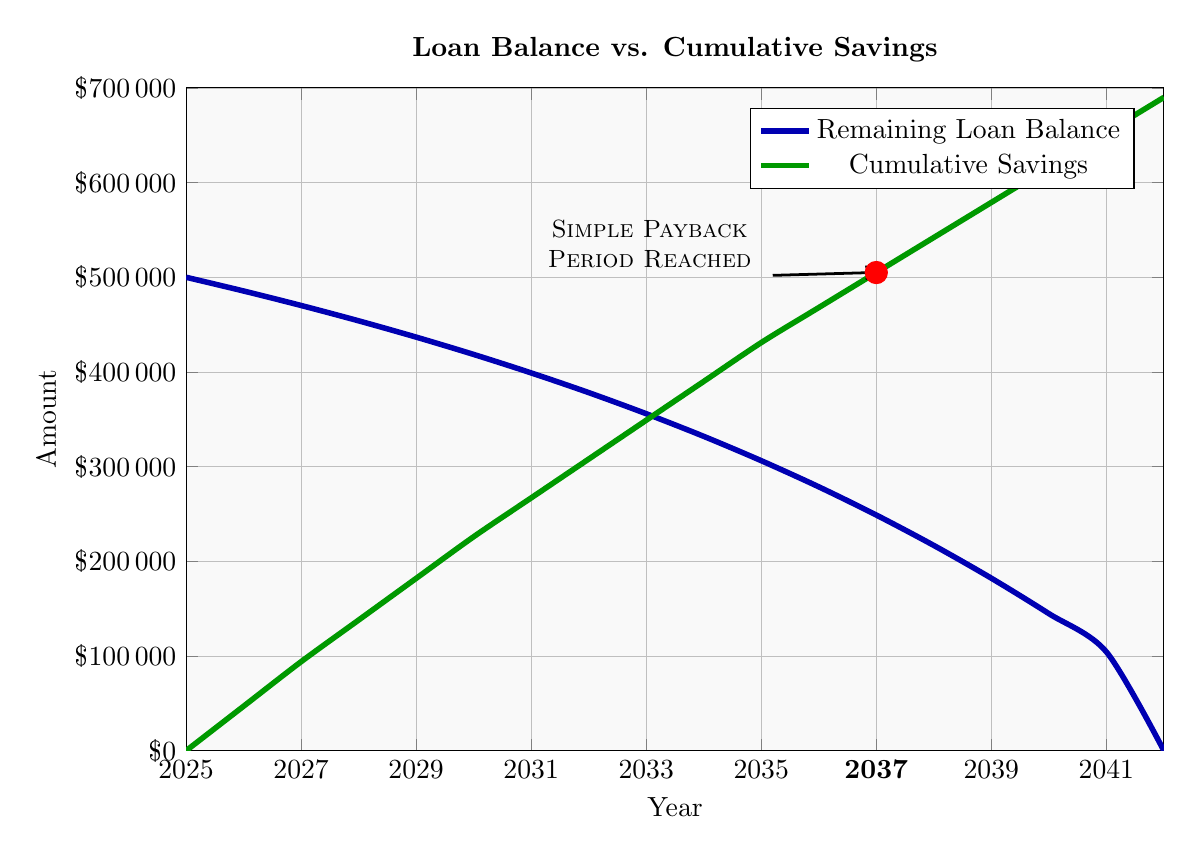
\begin{tikzpicture}
\begin{axis}[
    title={\textbf{Loan Balance vs. Cumulative Savings}},
    xlabel={Year},
    ylabel={Amount},
    xmin=2025, xmax=2042,
    ymin=0, ymax=700000,
    legend pos=north east,
    grid=major,
    grid style={line width=0.1pt, draw=gray!30},
    major grid style={line width=0.2pt, draw=gray!50},
    width=14cm,
    height=10cm,
    axis background/.style={fill=gray!5},
    scaled y ticks=false,
    y tick label style={/pgf/number format/fixed,/pgf/number format/1000 sep=\,},
    yticklabel={\$\pgfmathprintnumber{\tick}},
    xtick={2025,2027,2029,2031,2033,2035,2037,2039,2041},
    x tick label style={/pgf/number format/fixed,/pgf/number format/1000 sep=},
    xticklabels={2025,2027,2029,2031,2033,2035,\textbf{2037},2039,2041}
]

% Realistic loan balance with proper amortization curve
\addplot[color=blue!70!black, line width=2pt, smooth] coordinates {
    (2025, 500000) (2026, 485500) (2027, 470200) (2028, 454000) (2029, 436800)
    (2030, 418500) (2031, 399000) (2032, 378200) (2033, 355900) (2034, 332000)
    (2035, 306300) (2036, 278700) (2037, 248900) (2038, 216800) (2039, 182200) (2040, 144800) (2041, 104400) (2042, 0)
};

% Cumulative savings - higher annual savings that exceed loan principal
\addplot[color=green!60!black, line width=2pt, smooth] coordinates {
    (2025, 0) (2026, 47000) (2027, 94000) (2028, 138000) (2029, 182000)
    (2030, 226000) (2031, 267000) (2032, 308000) (2033, 349000) (2034, 390000)
    (2035, 431000) (2036, 468000) (2037, 505000) (2038, 542000) (2039, 579000) (2040, 616000) (2041, 653000) (2042, 690000)
};

% Add marker at payback point
\addplot[only marks, mark=*, mark size=4pt, color=red] coordinates {(2037, 505000)};

% Add professional annotation with arrow
\node[anchor=south east, align=center, font=\small\sffamily] at (axis cs:2035,500000) {
    \textcolor{black}{\textsc{Simple Payback}}\\
    \textcolor{black}{\textsc{Period Reached}}
};
\draw[->, color=black, line width=1pt] (axis cs:2035.2,502000) -- (axis cs:2036.95,505000);

\legend{Remaining Loan Balance, Cumulative Savings}

\end{axis}
\end{tikzpicture}
\end{center}

The simple payback period occurs when the green cumulative savings line reaches the loan principal amount of \$500,000. This visualization shows how cumulative savings continue to grow beyond payback, demonstrating the long-term financial benefits of the retrofit investment.

\section{Implementation Notes}

All variables in the codebase follow camelCase naming convention with the appropriate PTAC or PTHP suffix for clarity. The calculations are implemented in the backend services using TypeScript, ensuring type safety and consistent naming across the platform.

\end{document}